\documentclass[../xdudla00-porting-Tang-to-Open-WRT.tex]{subfiles}
\begin{document}

\chapter{Encryption}\label{encryption}

Nowadays, it is common to have a password protected system.
But the encrypted disk requires another password (key) to decrypt.
Imagine you come home in a mood to enjoy your time and your system asks for password, not once, but twice.
I think this is the reason why most of us do not use encryption, even when we know it will protect our data.
This is what \\Tang \ref{tang} is used for, since we want to automatize things.

Lets take a look on how the encryption is typically done.
As you can see in the image Figure \ref{fig:encdata} it all starts with desire to keep our data to ourselves and as a secret to the other people.
More often than not, these secrets are stored on our hard drives.
Usually we encrypt this secret by using an encryption key.
However, our secret data might grow in size, and it is time and resource consuming to decrypt and encrypt the secret every time encryption key changes or it is compromised.
Because of that, we wrap encrypted data in the key encryption key and this is what the system prompts from us when booting.
So, changing the key encryption key does not affect encrypted data.
We can change it whenever we desire to and redistribute the new key to all users who are supposed to access this data.

\begin{figure}[h]
    \centering
    %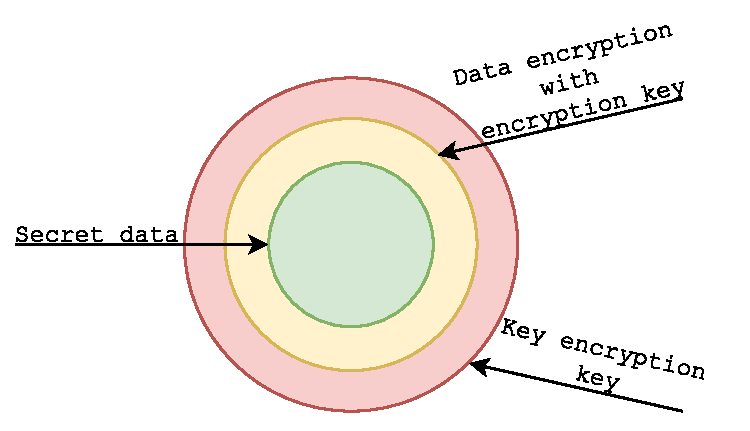
\includegraphics[scale=0.7]{../figures/HowWeEncryptData.pdf}
    \caption{How we encrypt data}
    \label{fig:encdata}
\end{figure}

To automatize this, we could generate something cryptographically stronger than user provided password.
Then, we store this cryptographically stronger random key on a remote system, from where we can get it later.
This is basically how the Escrow \ref{escrow} model works.

\end{document}
